\begin{tikzpicture}[remember picture]
    \begin{axis}[
        width=0.85\textwidth,
        height=0.63\textheight,
        xlabel={Time},
        ylabel={Price},
        title={Price over Time},
        legend cell align={left},
        legend style={font=\footnotesize},
        legend pos=outer north east,
        xtick=data,
        xticklabels={{1},{2},{3},{4},{5},{6},{7},{8}},
        ytick=data,
        yticklabels={{10},{11},{12},{13}},
        ymin=9.6,
        ymax=13.3,
        grid=both,
        grid style={line width=.1pt, draw=gray!10},
        major grid style={line width=.2pt,draw=gray!50},
        minor tick num=2,
        xmajorgrids=true,
        ymajorgrids=true,
        ]
        \addplot[mark=square*,blue] coordinates {
            (1,9.95)(2,11.15)(3,12.05)(4,13.05)(5,11.2)(6,12.2)(7,12)(8,11.7)
        };
        \addlegendentry{Actual Price};
        \addplot[mark=square*,red] coordinates {
            (1,9.8)(2,9.9)(3,9.9)(4,10)(5,9.8)(6,9.8)(7,9.9)(8,9.7)
        };
        \addlegendentry{T5+TimeS};
        \addplot[mark=square*,orange] coordinates {
            (1,9.8)(2,9.9)(3,9.9)(4,9.9)(5,9.9)(6,9.9)(7,9.9)(8,9.7)
        };
        \addlegendentry{D-Linear+W};
    \end{axis}
\end{tikzpicture}